\section{Metamodel Related Approaches} \label{sec:metaApproaches}
Metamodel related approaches describe the abstract language structure with a model for \emph{the language}, which conforms to a Metamodel \emph{for languages}. When the language model is used, an instance model of it is created. For example, the Unified Modeling Language \footnote{\raggedright \url{http://www.uml.org/}}  2 (UML2) from the Object Management Group \footnote{\raggedright \url{http://www.omg.org/}} formally defines besides the notation the structure of UML2 models in its Superstructure \cite{Uml23s}. The Superstructures structure is described using UML2 Infrastructure \cite{Uml23i}, which is also called Meta-Object Facility (MOF). The relationship of MOF to UML2 is similar to the relationship of BNF to a programming languages grammar.\\
One advantage of a metamodeling is that formal models or languages are created and that tools for supporting metamodels can be build, which integrated if they use a common meta Metamodel.\\

This section first explains the the relation of MOF with Ecore, the Metamodel of Eclipse Modeling Framework (EMF), and their interchange. Afterwards EMF in general is explained, following by a description of projectional editors based on EMF and then EMF related textual editing is addressed.

\paragraph{MOF versus Ecore}
Meta-Object Facility (MOF) is a modeling concept comparable to Ecore. It is defined by the Object Management Group \cite{OMG} to define UML2. Essential Meta-Object Facility (EMOF) is the lightweight core of MOF that closely resembles Ecore. EMF can read and write EMOFs serialization format. \cite{EMP}

\paragraph{XML Metadata Interchange (XMI)}
XMI is the standard serialization format of EMF models in XML. The "XMI format (...) could technically be considered a concrete syntax, although it's sometimes called a serialization syntax." \cite{EMP}


\subsection{Eclipse Modeling Framework (EMF) }
"EMF is a Java framework and code generation facility for building tools and other applications based on a structured (data) model" \cite{EMFDoc}. 
It does not depend on Eclipse. EMF unifies a subset of Java, XML and a subset of UML by models, which are definable using XML Schema, annotated Java interfaces or UML modeling tools. EMF bridges the gap between modelers and Java programmers by relating modeling concepts to a simple Java representation of these concepts. \cite{EMF2nd}\\

EMFs runtime framework\footnote{\raggedright The runtime framework distinguishes the part of EMFs framework from the one which is necessary for code generation.}  allows data to be validated, persisted and edited in an user interface editor. Change recording and notification as well as meta data by reflection is available. EMF is the foundation for fine-grained interoperability and data sharing among tools. For example Model Transaction \footnote{\raggedright \url{http://www.eclipse.org/modeling/emf/?project=transaction}}, graphical editors like the Graphical Modeling Framework GMF \footnote{\raggedright \url{http://www.eclipse.org/modeling/gmp/?project=gmf-runtime}}, database persistence \footnote{\raggedright \url{http://wiki.eclipse.org/Teneo}} , model transformation and so on.

EMF supports saving models to and loading them from persistent resources. A specialized XML serialization format called XML Metadata Interchange (XMI) is available as a default serialization. References can be persisted, they can be across multiple resources with load on demand, proxy resolution and unloading or proxy creation support. References can be bidirectional in EMF with referential integrity maintained. \cite{EMF2nd}\\

\subsubsection{Ecore Meta Metamodel} \label{ecore}
EMF uses a model to describe other EMF models. This model is called Ecore and is the center of the EMF world. \todo{"i.e. what node types are available and in which way they can be combined"?}. Ecore is itself an EMF model and can be described by itself similar to the possibility of describing the syntax of EBNF in EBNF. This makes Ecore its own metamodel, thus Ecore is a meta-metamodel. The concepts of metamodels is simple: a model which describes a model is a metamodel. A model which describes a metamodel is a meta-metamodel. \cite{EMF2nd}  A metamodel describes the abstract syntax of a language \cite{EMP} and the added validation rules the static semantics of a language \cite{MDSD}

Ecore supports several high level concepts which are not directly available in Java, like multiple inheritance, bidirectional relationships and containment relationships as a specialization of bidirectional relationships. Cycles in containment relations are forbidden and an \code{EObject} might just be contained in exactly one other \code{EObject}. Containment relations forms trees within models. The roots of these trees are model elements without container \code{EObject}, likely with a container \code{Resource} and the leafs are \code{EObject} without outgoing containment relations.  \todo{EObject base class, Object in java}

\begin{figure}
\centering
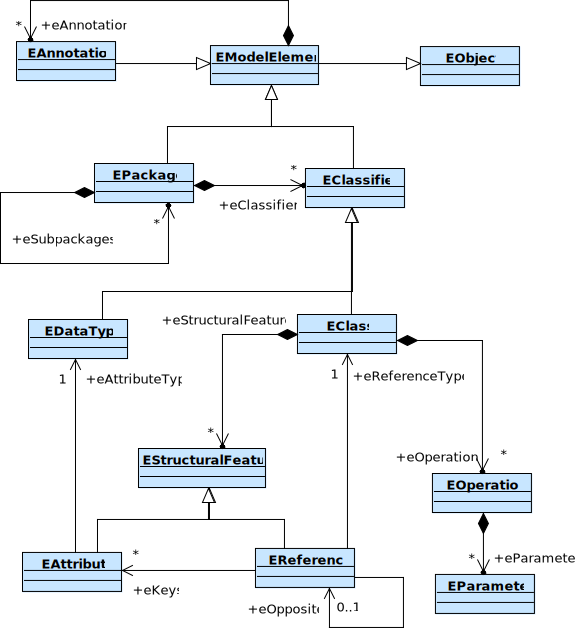
\includegraphics[scale=0.9]{gfx/ex/Ecore} 
\caption{Simplified Ecore Metamodel}
\label{MM:Ecore}
\end{figure}
	
Figure \ref{MM:Ecore} shows a subset of Ecore. \todo{Intro?} The central elements of Ecore are:\\
\begin{itemize}
	\item \emph{EObject} the common supertype of all Metamodel objects \emph{and} instance objects. \code{EObject} is similar to Objects in Java.
	\item An \emph{EPackage} is the root of an model and contains EClassifiers and subpackages.
	\item \emph{EClass} models classes. A class refers a number of other classes as its supertypes. They are identified by name and contain a number of attributes and references which both are structural features.
	\item \emph{EStructuralFeature} is the supertype of attributes and references, it aggregates attributes like multiplicity.
	\item \emph{EAttributes} have a type and are identified by name. They model the components of an objects data.
	\item \emph{EDataType} represents a single type which must not impose structure. They are directly related to Java types.
	\item \emph{EClass} and \emph{EData} types are both \emph{EClassifiers}.
	\item \emph{EReferences} model one end of an association. They are identified by name and hold a type of the referable object. If the association is bidirectional, the \emph{eOpposite} is assigned to its inverse reference. \cite{EMF2nd}
	\item Ecore classes hold and \emph{eAnnotation} reference. \emph{Annotations} store information which were not considered fundamental enough to explicitly support them in Ecores metamodel. For example documentation, OCL validation, XML serialization parameters. \cite{EMP}
	\item In additional to structural features, Ecore can also model the interfaces of behavioral features.
\end{itemize}

\paragraph{Generator model}
The generator model is the model that provides access to the data needed to generate the Ecore model by \emph{decorating} it. This separation has the advantage that the Ecore model can remain pure without code generation dependent information with the disadvantage that it might get out of sync \cite{EMF2nd}.


\subsubsection{EMF Runtime}
EMFs runtime framework provides the basis for manipulation, change notification and serialization of EMF objects in general. \cite{EMF2nd} Change notification is based on the observer pattern \cite{patterns}, which are called adapters in EMF, because they frequently extend behavior of \code{EObject}s and adapt them. The behavior of adapters must be described in Java, EMF just declares behavior but does not specify it. All \code{EObject}s are observable, but also other EMF classes like \code{Resource} are.

In the following, just the persistence part of EMFs runtime is described. EMF.Edit, which is also part of it is explained separately in the Projectional Editors section. XText \cite{XTextMan} and EMFText \cite{EMFTextMan} integrate themselves in EMF as \code{Resource}, which is part of EMFs persistence concept. Resource, and ResourceSet are fundamental interfaces of EMFs persistence framework.

\paragraph{Cross Resource References}
To reference other persisted objects EMF uses Proxies. A Proxy is an uninitialized instance of the target class, which is identified by an URI. " A Uniform Resource Identifier (URI) is a compact sequence of characters that identifies an abstract or physical resource." \cite{URI} A URI consists of five parts: scheme, authority, path, query and fragment whereby query is not considered for this thesis. The basic format is:\\
\code{schema://authority/path\#fragment} \\
The schema defines the interpretation of the following part. Common schemata for EMF are file, in an eclipse environment platform and http. Authority and path together identify an resource, the fragment identifies a part of an resource or in the case of EMF an \code{EObject}.\\
For example:\\
\code{http://www.xtext.my/MiniJava\#//@class.1}\\
which identifies the the second element stored in the containment reference \code{class} of the resource \code{http://www.xtext.my/MiniJava}.


\paragraph{Resource}
A resource is a basic unit of persistence. It is a container for one or more objects which are persisted together with their children. They can be unloaded, in which case contained referred objects  are converted to proxies. An resource is identified by a URI with schema, authority and path. A resource is also responsible for creating valid URI fragments for \code{EObject}s it contains. By default a resource returns hierarchy based XPath like fragments. Other options are intrinsic IDs and extrinsic IDs. Intrinsic IDs are IDs stored directly on the model object, whereas extrinsic IDs are stored external of the object. Extrinsic IDs are useful when the modeled objects state is not sufficient to constitute an ID for a given resource. XML resources manage extrinsic IDs and offer support for universally unique identifiers (UUIDs). It is possible to attach adapters to a resource, so it is for example possible to observe every change of an contained object and create a \code{ChangeModel} by using EMFs \code{ChangeRecorder}. This enables automatic undo support for commands. \cite{EMF2nd}.

\paragraph{ResourceSet}
A ResourceSet acts as a container for Resources and its main responsibility is to support references between objects in different resources. 

\subsection{Projectional Editors}
This section describes two projectional editors for EMF models, EMF.Edit and the Graphical Modeling Framework (GMF). EMF.Edit is a framework for tree and table editors, whereas GMF is a full graphical editor.

\subsubsection{EMF.Edit}
With EMF Edit it is possible to build editors for models, which display and edit (i.e. Copy, drag-and-drop, etc.) model instances with unlimited undo and redo. EMF.Edit is the controller in the MVC pattern which uses JFace, a SWT based user interface toolkit, viewers by default. EMF.Edit and GMF controllers are in between view and model, so the view has no direct connection to the model. EMF.Edit supports object modification based on the Command pattern \cite{patterns} and includes a number of common commands. A command offers execute, undo, redo and canExecute to check if all constraints are satisfied.  EMF.Edit includes a set of generic commands based on the reflective API like Set, Add, Remove, Move, Replace and Copy, as well as  higher level commands like CreateChild, DeleteChild, CutToClipboard, CopyToClipboard, PasteFromClipboard and DragAndDrop. Controllers are called ItemProviders im EMF.Edit, they offer to navigate their structure, modify their content, to retrieve labels, to forwards notifications to the viewer as well as acting as a command factory. Controller are in general associated with an EObject, but do not need to, in order to let the editor display a structure different from the models structure. The central unit of EMF.Edit is the EditingDomain which encapsulates a ResourceSet, adds a command stack to support undos and redos as well as provides a controller factory \cite{EMF2nd}. EMF.Edit also provides a reflection based generic editor for \emph{any} Metamodel instance.  


\subsubsection {Graphical Modeling Framework (GMF)}
GMF is a framework for creating graphical eclipse editors that are based on an EMF model. It's a controller framework using EMF Models for persistence and Draw2D as View. GMF is based on GEF \todo{ausschreiben, link} and unifying GEF and EMF commands and extensively uses eclipse extension points. Furthermore it adds a notation model, which persists layout information independent from the language metamodel and model. The concept of a Notation Model is explained in detail \todo{really, in detail?} and how it is integrated in GMF. The main purpose of GMF, the controller, is skipped because the much simpler controllers of EMF.Edit are sufficient in the context of this thesis. To bridge the gap, it's important to note that GMF creates a controller for each View, that is the basic model element of the notation model. Creating more than one View e.g. by the view service factory is a common practice in GMF to separate the presentation structure from model structure. Which view should be created is hinted by the Extensible Type Registry.

\paragraph{Notation Model}
GMFs notation model manages and persists the state of the diagram or view separated from the language model. It is completely domain model independent and thus can be handled generically by GMFs engine to provide common features. It manages the diagram element, position and style attributes. \cite{EMP} The base type of the notation model is View, which:
\begin{itemize}
	\item holds a reference to the language model element it represents 
	\item acts as the super type for node, edge and the notation models root: diagram
	\item contains child nodes and refers to edges
	\item has attributes like visibility and type
\end{itemize}

\begin{figure}
\centering
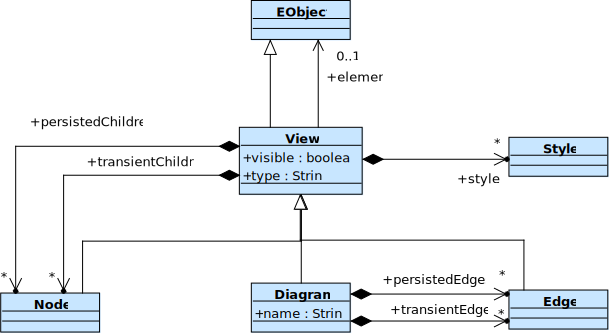
\includegraphics[scale=0.8]{gfx/ex/GMF_Notation} 
\caption{Simplified GMF Notation Metamodel}
\label{MM:GMF}
\end{figure}

Part of the design considerations for the notation meta model were \cite{GMFDoc}:
\begin{itemize}
	\item The notation meta-model was designed to minimize merging conflicts through the separation of style into granular properties. They can be merged independently.
	\item The style hierarchy has been designed to be extend able. The allows individual extensions and enhancements in the future. 
\end{itemize}

\paragraph{View Service}
The View Service is a factory for constructing new notation view elements also based on \cite{GMFDoc}:
\begin{itemize}
	\item the corresponding language element (EObject)
	\item the type determined by the Extensible Type Registry.
	\item the container view  
\end{itemize}

\paragraph{Extensible Type Registry}
``The Extensible Type Registry provides a way for GMF clients to define an application-specific classification system based on, but alternative to, the metaclasses defined by an Ecore metamodel'' \cite{GMFDoc}. This means that it is possible to introduce specialized GMF internal types, e.g. on the state of the referred EObject or the state of another EObject referring the current one.








%%%%%%%%%%%%%%%%%%%%%%%%%%%%%% EMF () %%%%%%%%%%%%%%%%%%%%%%%%%%%%%%%%%%%%%%%%%%%%


 

\subsection{Textual Editing}
This section describes how textual is integrated in EMF. At the beginning, the relationship between context free grammars and MOF based Metamodels is described. In the following Xtexts \cite{XTextMan} grammar and Xtexts architecture is described. EMFText \cite{EMFTextMan} is besides Xtext the other well documented, still active developed textual framework for EMF. In contrast to Xtext, it allows to automatically derive a textual notation from a Metamodel and layout information in grammar rules. From the abstract point of view of this thesis, the are similar except that EMFTexts documentation does not indicate how isomorphism from EClass to grammar rule can be circumvented. The relevance of this is discussed in \todo{link}. This section closes with the editing strategy of Textual Editing Framework (TEF).


%%%%%%%%%%%%%%%%%%%%%%%%%%%%%%%%%%%%%%%%%%%%%%%%%%%%%%%%%%%%%%%%%%%%%%%


\subsubsection{Relation of Metamodels and Context Free Grammars} \label{sec:MM:CFGs}
To connect the textual languages, which are typically denoted by context free grammars and modeling languages, which are described by metamodels, a mapping between the concepts of BNF and Ecore has to be established. Because Ecore is more expressive than BNF, it is possible to map BNF to Ecore, but just a subset of Ecore to BNF.

Algorithms for mapping a subset of MOF to BNF and BNF to MOF are described in \cite{MofCfg}. Note that \cite{MofCfg} uses a subset of MOF which is also a subset of Ecore and uses enumerations for fixed string literals (keywords), which is an optional specialization of the presented attribute mapping. Also,  \cite{MofCfg} maintains an attribute order by generating lexical ordered structural feature names. Whereby an attribute order is crucial, this is not necessary regarding Ecore. EMF implements unordered multiple values as lists, which are ordered. This implementation characteristic is documented \cite{EMF2nd}.  \cite{MofCfg} mentions that it's possible to create "invalid" models of the grammar metamodel, which requires additional verification with the target context free grammar. This topic is discussed later in \todo{ Example?}

The general idea of context free grammars to Metamodels mappings is:
\begin{enumerate}
	\item Each production rule creates an (abstract) class.
	\item For each alternative,  a subclass of the production rules class is created.
	\item Every non-terminal is mapped to a containment reference of the created (abstract) type of the production rule(s) for that non-terminal.
	\item Every terminal is mapped to an attribute.
\end{enumerate}

The mapping is straightforward, just the alternative to subclass mapping might surprise at first glance. Choices and subclasses both represent exchangeability. The 3. and 4. step are mixed to contain the symbol order.

Mapping Metamodels to context free grammars adds the problem of representing cross-references for which there is no correspondence in BNF. They can however be represented as terminals identifying the referenced element.   

This mapping defines the foundation to bridge between Metamodels and context free grammars. It describes how a model represents a Parse Tree. The Parse Tree is bound by the concrete textual syntax. In general however, Ecore models describe the abstract syntax of a language and not the Parse Tree of one textual representation. To gain more flexibility, the EBNF description is enriched by an synthesized attributed grammar which defines the AST. The mapping between S-attributed Grammar and Ecore will be described after a discussion of XTexts grammar.
%%%%%%%%%%%%%%%%%%%%%%%%%%%%%%%%%%%%%%%%%%%%%%%%%%%%%%%%%%%%%


\subsubsection{XText Grammar}
XTexts grammar language is a domain-specific language to describe textual languages. The main idea is to describe the concrete syntax and its mapping to an in-memory representation - the ``semantic model''. Xtext supports grammar mixins, which is the reuse of existing grammars. It can infer Ecore models from a grammar, but it's also possible to import existing Ecore models instead. In the following, the XText grammar will be explained by example in conjuction with the optional Ecore inference. The metamodel created by inference helps understanding how Metamodel and synthesized attributed EBNF constrain each other. In case of the manually maintained metamodel, this metamodel must follow certain constraints. Based on the Liskovs substitution principle, the classes of the manual metamodel must be a substitute of the classes of the inferred metamodel which would have be created. In case of model inference the created structural features are normalized, meaning if all subclasses share a features with the same name, type and multiplicity they are merged together in the common superclass.

XText uses an EBNF with the following notation extensions:
\begin{itemize}
	\item Option, meaning one or none is denoted by '?'
	\item Any, meaning zero or more is denoted by the Kleene star '*'
	\item One or more is denoted by the Kleene cross '+'
	\item Keywords are enclosed in ``'' or '', e.g. ``keyword'' or 'anotherKeyword'
	\item Grouping is possible by enclosing brackets '(' and  ')', e.g.  ( A b C)
\end{itemize}

\paragraph{Lexer Rules}
In XText there are Lexer rules,  which extend the EBNF notation by:
\begin{itemize}
	\item Character Ranges, which are denoted by start character '..' stop character, e.g. '0'..'9' 
	\item Wildcards, which allow any character are denoted by '.'
	\item Negation, denoted by '!'
	\item the end of file token, denoted by 'EOF'
	\item Until token, which consumes everything until the stop token occurs is denoted by '->', e.g. '/*' -> '*/'
\end{itemize}
A terminal rule looks like for example:
\begin{xtxt}
terminal SL_COMMENT : "//" !'\n'* '\n';
\end{xtxt}
this is equivalent to 
\begin{xtxt}
terminal SL_COMMENT returns ecore::EString : "//" !'\n'* '\n';
\end{xtxt}
The return type is optional and by default EString. The order of terminal rules is important, because they shadow each other. Terminal rule names are written in capital letters as a naming convention. Terminal rules are mapped to the data type following the returns keyword and are converted to it using the ValueConverters.

\paragraph{Parser Rules}
A parser rule produces a tree of terminal and non-terminal tokens and all parser rules together produce the Parse Tree, which is also referred as Node Model in Xtext. Additionally, parser rules are the building plan for the creation of EDataTypes or EObjects which form the AST. XText also calls the AST semantic model. EObjects are created lazy by default. Actions and assignments are used to derive types, to force their instance creation and to build the AST accordingly. The first parser rule in the grammar is the start production. It's possible to hide terminal tokens from the parser, like comments. Hidden tokens are ignored in the parser, but should be preserved during deserialization.

\subparagraph{DataType Rules}
Data type rules are parsing-phase rules, which return EDataTypes. They are similar to terminal rules, but because they are parser rules, they are context sensitive. Rules that don't call parser rules, nor contain actions or assignments are considered data type rules with the default return type EString. 
\begin{xtxt}
Number returns ecore::EInt : NUM ('.' NUM*)?;}
\end{xtxt}

\subparagraph{Assignments}
Assignments are the synthesized attribution of the EBNF dialect. They assign the information of a consumed symbol to the structural feature of the currently produced object. E.g.:
\begin{xtxt}
Person : "Person" age=Number;
\end{xtxt}
This creates a Metaclass named Person with an attribute named age of type EInt. 
The type of the current object(a subtype of EClass) is the return type of the parser rule. The types name is equal to the rules name by default.
\begin{xtxt}
Person : "Person" ("alias:" aliases+=ID)+;
\end{xtxt}
This rule creates a multi-valued structural feature for aliases and adds each ID occurrence to it. Also '?=' exists which assigns true to a boolean value if the right side was consumed.
\begin{xtxt}
Class : "class" (public?="public")?
\end{xtxt}
The right hand side of an assignment can be a rule call, a keyword, a cross-reference or an alternative composed by the former. It is also possible to specify the type of the returned \code{EObject} of a rule explicitly using \code{returns}. The previous rule is equal to:
\begin{xtxt}
Class returns Class : "class" (public?="public")?
\end{xtxt}

\subparagraph{Unassigned Rule Calls}
If a rule does not contain any assignments, but calls Parser Rules, it's called an unassigned rule. The return type of this rule is an abstract class, which has to be a supertype of returned types of TokenA, TokenB and TokenC. Xtext generates an abstract class named \code{AbstractToken} for this example by default.
\begin{xtxt}
AbstractToken :	TokenA |	TokenB |	TokenC
\end{xtxt}


\subparagraph{Linking}
Xtext allows the declaration of cross-references in the grammar as terminal tokens, but not the linking semantics because of its synthesized attributed context free nature. The actual resolving process is done programmatically and not of interest, for this thesis. The general idea is discussed in \ref{sec:xtextarch:Linking} \todo{name}
e.g. 
\begin{xtxt}
Reference:  "Ref" event = [MyEvent| VALID_EVENT_ID]
\end{xtxt}
It's important to note that MyEvent is the referenced types EClass, not a parser rule. The  \kode{|VALID_EVENT_ID} is optional and refers to an EDataType rule or uses a string by default.

\subparagraph{Enumeration Rules}
Enumeration Rules convert between enumeration literals and strings and are a shortcut for data type rules with specific value converts.

\subparagraph{Actions}
The returned object with its type can be explicitly controlled with actions. Xtext supports two kind of actions, simple actions and assigned actions. Simple actions explicitly instantiate the \code{EObject}s type of the current choice using the notation \kode!{EClass_aka_EObjectType_To_Return}!.
\begin{xtxt}
Z 	: 	{B} "A" v=ID
	| 	{C} "B" v=ID;
\end{xtxt}
Xtext requires and infers that \code{B} and \code{C} are subtypes of \code{Z}. 

Assigned actions are used for tree rewriting which is necessary to cope with shortcomings of the underlying parser technique. Because XText uses the ANTLR parser generator framework, which is based on the LL(*) algorithm, it can't handle left recursive grammars. It is therefore necessary to rewrite or 'massage' the grammar, which is called "left-factoring" in the case left recursion is dissolved. Because this left-factoring ends in an unwanted AST, it is possible to rewrite the tree by assign the current EObject to a structural feature of the returned EObject, e.g. 
\begin{xtxt}
Expression 	: 	LExpression 
	 	( "&&" {And.left=current}  right=Expression)
\end{xtxt}
whereas \kode{And.left=current} is the tree rewrite action which assign the element currently-to-be-returned (\kode{current}) to the structural feature \kode{left} of the newly created element \kode{And}.


\subparagraph{Syntactic Predicates}
XText offers the possibility of syntactic predicates, which are necessary to solve ambiguity, like the dangling else problem and also help in cases where grammar rewriting would be necessary otherwise. Syntactic predicates are a specialization of semantic predicates regarding the underlying parser generator framework ANTLR. Syntactic predicates enable backtracking for a local scope and is enabled in XText by \code{=>}.


\subsubsection{XText Architecture} \label{cha:xtextarch}

\paragraph{Value Converters}
Because Xtext translates between an abstract syntax tree and a stream of characters in both directions, the sequence of characters inevitably has to be converted to a proper data type and vice versa. This bidirectional transformation is the job of \code{ValueConverter}s and is done by two (inverse) unidirectional transformations. Converters are used by the Lexers Terminal Rules and Parser Rules.


\paragraph{XText Phases during deserialization}
The parsing process in XText is separated into following phases:
\begin{enumerate}
	\item Lexing and Parsing: The lexing phase transforms a sequence of characters into tokens. Tokens are a strongly typed part of the input sequence. Their represent an atomic symbol and their type is determined by a particular terminal rule or keyword. The parsing phase requests tokens and builds a ParseTree and an AST according to the grammar rules.
	\item Linking resolves the textual identification of ``referrenced'' targets to Cross References after parsing is complete.
	\item The Validation Phase is optional.
\end{enumerate}

This section describes how XText realizes the \todo{Np concepts} concepts described by the grammar. It focuses on Parsing, Unparsing, the gap between abstract syntax and parse tree, Referential Integrity. \todo{sounds like shit AND is now wrong}

XText converts the input grammar to an EMF model, saves it and provides helper methods for runtime grammar access. XText integrates itself in EMF as a Resource named \code{XTextResource}, which is shown in figure \ref{XtextArch}.  The basic components of a XText resources are the Serializer, to convert EObjects to text, the Parser, to convert text to EObjects or to deserialize the EObjects and the Linker which manages Cross-References. 

\begin{figure}
\centering
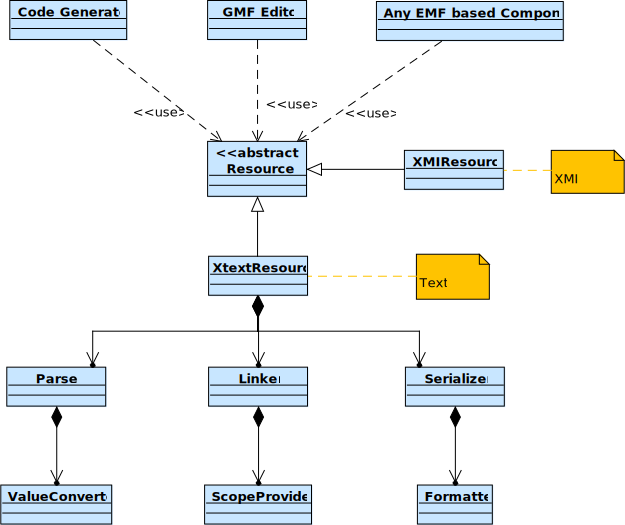
\includegraphics[scale=0.75]{gfx/ex/Xtext} 
\caption{XtextResource Implementation, based on \cite{XTextMan}}
\label{XtextArch}
\end{figure}
The main drawbacks of this solution are:
\begin{itemize}
	\item During incremental changes, the XText parser replaces subtrees instead of updating them, so existing EObjects become stale. The XText documentation advices against the use of a "self-synchronizing (...) editor" on the same model as XText but suggests working on a copy.
	\item The implementation to identify EObject in a resource has to return stable fragments.
\end{itemize}

\paragraph{Parsing}
XText uses ANTLR \cite{ANTLR} for parser creation. It creates ANTLR grammar files with ANTLR Grammar Actions to create the AST and ParseTree. The rules return EObjects, 'init' and 'after' actions are used as guidance of the current stack position for the creation of nodes. The returned EObjects form the AST and related to them, a node model is created which is related to the AST. 

\subparagraph{Node Model}
The node model is created during parsing. The term ``node model'' is defined by Xtext and does not conform to the model definition of this thesis, because no metamodel exists. The base interface of the node model is INode which  is described as "A node in the parse tree" \cite{XTextAPI}. Nodes are either composite nodes if they represent non terminals or leaf nodes, if they represent terminals. Nodes hold a reference to the grammar element they represent and leafs to the represented token additionally. Nodes are added to the EObjects as Adapters instead of referring to them by an EReference.

The roles of the node model during serializations are:
\begin{itemize}
	\item preserves existing white spaces
	\item preserves existing comments
	\item preserves the representation of cross-references, in case multiple names are possible
	\item preserves the representation of values, in case multiple representations are possible, e.g. 1.0, 1.00, 1.000.
\end{itemize}

\paragraph{Linking}
\label{sec:xtextarch:Linking}
Linking of Cross-References by means of textual identifiers can be separated into two parts:
\begin{itemize}
	\item how XText copes with the mismatch between cross references and text in general. In this case, just inner resource references are considered. 
	\item how does XText resources cope with integration in EMF as an EMF resource.
\end{itemize}
The general idea of linking in XText is that every grammar rule which contains a reference is visited after the ANTLR parser \todo{explain ANTLR} finished. While visiting the AST, an ILinker instance is consulted to resolve each link. How the link is resolved is specified by the language designer by programmatically, using the textual representation saved in the node model and the context, which is EObject holding the reference which has to be resolved. XText strongly encourages the usage of a lazy linkers, which replaces the link with an EMF proxy containing the proper URI.

Beside the option to export just a subset of XTexts created EObjects, to achieve full EMF integration every EObject has to be referable, so the resource must be able to return the URI fragment of the given contained EObject and the EObject for a URI fragment. By default, XTexts Fragment Provider  uses path fragments like \kode{//@classes.0/@methods.0/@localVariables.3/@name}. XTexts documentation states that path references are fragile and that UUIDs should not be used regarding the users. 

\paragraph{Concrete Syntax Validation Constraints}
As mentioned in \cite{MofCfg}, it is possible to create invalid metamodels, where no valid textual representation can be deduced, even if the metamodel was inferred from the EBNF. The concrete syntax validation constraints described the how the grammar rules constrain a model, so it can be turned into word. They are used to validate if a textual representation is possible and also used to guide the serialization process to distinguish between different production and grammar rules, e.g.
\begin{xtxt}
Z 	:  "A" v=ID  
	|  "B" n=INT;
\end{xtxt}
given an instance of 'Z', it depends on if 'v' or 'n' is assigned to properly serialize 'Z'.
Given the rule
\begin{xtxt}
MyRule:	({MySubRule} "sub")? (strVal+=ID intVal+=INT)*;
\end{xtxt}
several constraints are implied:
\begin{enumerate}
	\item types: just instances of MyRule and MySubRule are allowed. Further specialized Subtypes are prohibited. 
	\item Features: if other structural features besides strVal and intVal exist, they must be either transient, unassigned or contain the default value.
	\item Quantities: the size of strVal and intVal must be equal.
	\item Values: all values must be convertable to valid terminal tokens.
\end{enumerate}
These constraints are created per production rule, not only per grammar rule. In case of 'Z' two independent set of constraints are created, one for the production starting with "A" and one for the production starting with "B".
XTexts concrete syntax validation is not capable of regarding:
\begin{enumerate}
	\item assigned actions, e.g. 
	\kode!{MyType.myFeature=current}!
	\item unassigned rule calls to assigned actions
	\item the order within list features, e.g. In \kode{Rule: (foo+=R1 foo+=R2)*} foo must contain R1 and R2 in alternating order
\end{enumerate}

\paragraph{Serialization}
The serialization process complements parsing and lexing by transforming EMF models into its textual representation. The XText documentation mentions six relevant steps:

\begin{enumerate}
	\item Validation
	\item Matching model elements with grammar rules by the parse tree constructor
	\item Associating comments
	\item Associating existing nodes
	\item merge white spaces and line wraps
	\item adding white spaces by the formatter
\end{enumerate}

In this thesis, only the parse tree constructor is discussed because:
\begin{itemize}
	\item validation is optional and is done with less meaningful error messages by the parse tree constructor
	\item comments, white spaces, line wraps are layout information without grammar relation.
	\item Runtime analysis showed that the existing node model is already accessed by the parse tree constructor, which indicates a gap in documentation and implementation.
\end{itemize}

\paragraph{Serialization contract}
"The contract of serialization says that a model which is saved (serialized) to its textual representation and then loaded (parsed) again yields a new model that is equal to the original model."\cite{XTextMan}

The following must hold:\\
I) $load(save(model)) \rightarrow model$\\
The inverse does not always hold, thus:\\
II) $save(load(text)) \nrightarrow text$\\
If the node model still exists, II) holds in most cases. 

Given the XText example, that for the following rule first all xvals and then all yvals will be written to the token stream.
\begin{xtxt}
MyRule: (xval+=ID | yval+=INT)*; 
\end{xtxt}
This indicates that XText follows the EObject containment order instead of the one of the node model.

\paragraph{Parse Tree Constructor}  \label{xtxt:ptc}
Actually the Parse Tree Constructor does \emph{not} construct nodes of the node model, it finds valid grammar rules for each EObject of the AST. 

It succeeds if all EObjects are visited and no concrete syntax validation constraint is violated. So the Parse Tree Constructor has to find a valid allocation for the traversed AST in which all grammar constraints hold.  This is, like parsing, a constraint satisfaction problem. XText solves this constraint satisfaction problem using top down backtracking, which results in potential exponential runtime of the serialization of a model. This is done by the Parse Tree Constructor finding valid 'paths' from the root to a leaf node constrained by the grammar. The Parse Tree Constructor stops after the first valid solution has been found. 

If there is no representation of a choice in the AST, a default needs to be specified, for example in the case: 
\begin{xtxt}
PluralRule: "contents:" count=INT Plural;
terminal Plural: "item" | "items";
\end{xtxt}
it is unclear during parse tree construction if 'item' or 'items' should be used. This case is named unassigned text in XText.



%%%%%%%%%%%%%%%%%%%%%%%%%%%%%%%%%%%%%%%%%%%%   TEF %%%%%%%%%%%%%%%%%%%%%%%%%%%%%%%%%%%%%%%%%%%%
\subsubsection{TEF - Textual Editing Framework}
With TEF it is possible to integrate textual editing in an existing MVC editor. This is done by selecting an element, showing its textual representation in an extra overlay and execute the changes when the overlay is closed. 
The basic steps are:
\begin{enumerate}
	\item Copying the selected element and all its directly and indirectly contained elements.
	\item Create a initial representation in an overlay text editor using backtracking.
	\item Use background parsing to constantly create new models at the location of the copy.
	\item Replace the edited model element if the overlay was closed.
\end{enumerate}

\begin{figure}
\centering
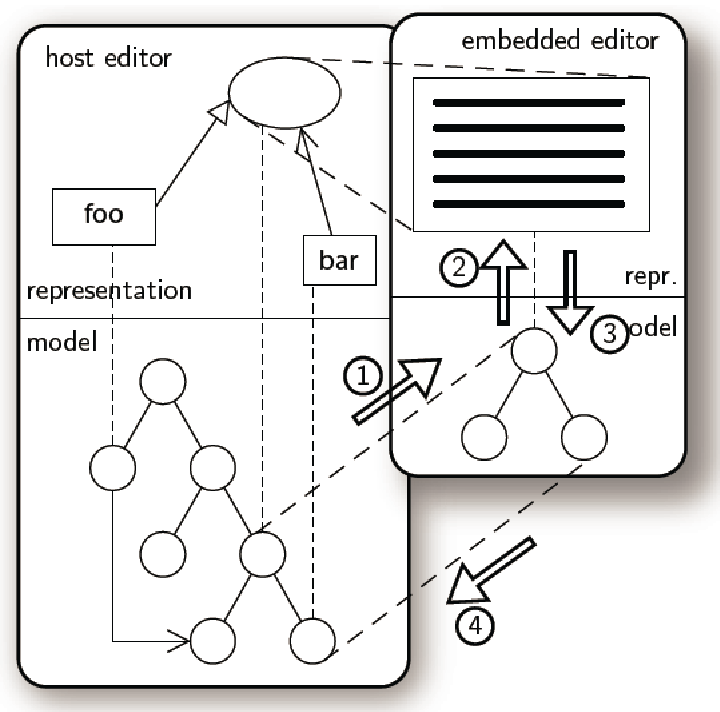
\includegraphics[scale=1.2]{gfx/ex/tef} 
\caption{Steps involved in the embedded textual editing process, from \cite{TefPaper}}
\label{pic:tef}
\end{figure}

Replacing has two fundamental problems:
\begin{itemize}
	\item all references to the replaced element break.
	\item Information which is contained in the original model, but not displayed in the textual representation is lost.
\end{itemize}
In order to solve the problems by reassigning the references and merging the models, identification is required. \cite{TefPaper} demands language-specific identification. 

TEF does not require the whole model to be describable textually, only the elements and it's directly or indirectly contained elements which should be textually displayable must be specified using a context free grammar.

TEF creates a Parse-tree from the model by traversing the model along its composition and determines a set of suitable grammar rules based on constraints. It uses backtracking for that and \cite{TefPaper} also suggest to enable the language engineer to prioritize grammar rules if multiple parse trees are possible.